\cotefile{157-1}
\scanpage{2}

Dérivateurs.

\diagram{\begin{tikzcd}[ampersand replacement=\&,row sep=2pt,column sep=4pt]
\overline{\underline{\mathrm{I}}}\arrow[dddddddddd,leftrightarrow,bend right=35] \& \parbox[t]{.69\linewidth}{Généralités sur les (pré)dérivateurs} \\
{[\overline{\underline{\mathrm{II}}}]} \& \parbox[t]{.69\linewidth}{Cofinalité (à droite et à gauche) (préliminaire à la cofinalité \unsure{cohomologique|cohomologiques})} \\
\overline{\underline{\mathrm{III}}}\arrow[dd,leftrightarrow,bend right=45] \& \parbox[t]{.69\linewidth}{Hom internes dans les dérivateurs} \\
\overline{\underline{\mathrm{IV}}} \& \parbox[t]{.69\linewidth}{Diagrammes substantiels} \\
\overline{\underline{\mathrm{V}}}\arrow[dd,leftrightarrow,bend right=45] \& \parbox[t]{.69\linewidth}{Catégories de \unsure{Chemins|chemins} et \unsure{localisation|localisations}} \\
\overline{\underline{\mathrm{VI}}} \& \parbox[t]{.69\linewidth}{HOT} \\
\overline{\underline{\mathrm{VII}}} \& \parbox[t]{.69\linewidth}{Catégories de chemins (2)} \\
\overline{\underline{\mathrm{VIII}}} \& \parbox[t]{.69\linewidth}{1-types d'homotopie relatifs\unsure{ :.| :} leur \unsure{intégration}\ldots} \\
\overline{\underline{\mathrm{IX}}} \& \parbox[t]{.69\linewidth}{Retour sur les $MW^{-1}$, comparaison avec Quillen} \\
\overline{\underline{\mathrm{X}}} \& \parbox[t]{.69\linewidth}{Comparaison de $\mathrm{Cat}$ avec $\unsure{\mathbb{\Delta}|\Delta}^{\wedge}$} \\
\overline{\underline{\mathrm{XI}}} \& \parbox[t]{.69\linewidth}{Hot-fibrations, foncteurs propres et foncteurs lisses etc. (dans $\mathrm{Cat}$)}
\end{tikzcd}}

$\overline{\underline{\mathrm{XII}}}$ Caractérisation de $W_{\infty}$. Foncteurs $W$-propres, $W$\unsure{.|-}lisses etc. bonnes \unsure{amalgamations} et carrés $W$-\unsure{cocartésiens} dans $\mathrm{Cat}$.

$\overline{\underline{\mathrm{XIII}}}$ \margin{?}Catégories de modèles (\unsure{1.|1|!})

$\overline{\underline{\mathrm{XIV}}}$ Carrés $h$-cartésiens et $h$-cocartésiens

$\overline{\underline{\mathrm{XV}}}$ \margin{?}Théorèmes de factorisation et Modèles \unsure{(2.))|(2.)}

$\overline{\underline{\mathrm{XVI}}}$ \deleted{\unsure{catég.}}\;Localiseurs fondamentaux dans $\mathrm{Cat}$

$\overline{\underline{\mathrm{XVII}}}$ \margin{?}Catégories à fibrations et à cofibrations. (Modèles \unsure{(3.)|(3))})

$\overline{\underline{\mathrm{XVIII}}}$ Catégories et ensembles accessibles.

$\overline{\underline{\mathrm{XIX}}}$ \margin{\unsure{?|1}}Modèles \unsure{(4.)|(4)}

% margin note written sideways
\margin{sont regroupés dans \unsure{chemise|même} \unsure{modèles|modèle} \unsure{1, 2, 3, 4}.}

\figure{\begin{tikzpicture}\draw[gray,->] (0,.95) -- (.67,0);\end{tikzpicture}}

% archive sheet number: 1
\scanpage{3}

$f^{!}$ existe-t-il pour $\unsure{X|x}\unsure{\longrightarrow|-}e$ ? (pour les dérivateurs habituels.)

% archive sheet number: 2
\scanpage{4}
\mspage{1}

\uline{Dérivateurs}

1. Préliminaires sur les foncteurs \unsure{image|images} \unsure{inverse|inverses} des préfaisceaux sur des catégories d'indices, et leurs adjoints multiples.

$A$ ``catégorie de coefficients''

$I$ ``catégorie d'indices'',

\[
A(I)=\underline{\mathrm{Hom}}(I^{\unsure{\circ|o}},A)\qquad\text{préf. sur }I\ \text{à valeurs }A
\]

Si $f:I\longrightarrow J$, on en déduit

\[
f^{*}:A(J)\longrightarrow A(I)
\]

\deleted{\unsure{E}}Et on s'intéresse à l'existence des foncteurs adjoints successifs à gauche et à droite. Notations provisoires

\[
f^{?}\ f_{!}\ f^{*}\ f_{*}\ f^{!}
\]

Voici les faits principaux :

a) Sous réserve de l'existence des $\varprojlim$ (resp $\underset{\unsure{-|\to}}{\lim}$) pertinentes, $f_{*}$ (resp $f_{!}$) existe. Par exemple s'il existe $\varprojlim$ (resp. $\varinjlim$) \uline{finies}, alors $f_{*}$ (resp. $f_{!}$) existe si $I,J$ sont des catégories finies.

b) Même si $A$ est une catégorie abélienne, \unsure{avec} $\varprojlim$ et $\varinjlim$\textsuperscript{*},\margin{* p. ex. \unsure{(Ab)}} les \uline{bi-adjoints} n'existent pas toujours\unsure{,|.} \deleted{\unsure{cf.}} \deleted{\unsure{déj.}} dans le cas particulier où $J=e$ est la cat. ponctuelle, et $I$ l'ens ordonné

\diagram{\begin{tikzcd}[ampersand replacement=\&]
\& a \\ \unsure{0|o}\arrow[ur]\arrow[dr] \& \\ \& b
\end{tikzcd}}

(dans le cas de $f_{\deleted{*}}^{!}$), ou l'ens ordonné opposé (dans le cas de $f^{?}$). Même si \deleted{c) Par contre, si} $f$ est une immersion \unsure{ouvert|ouverte}, $f^{!}$ n'existe pas forcément (par ex. \inserted{\unsure{définie par|déterminée par}} si $I$ comme dessus, et

\diagram{\begin{tikzcd}[ampersand replacement=\&]
\& a \arrow[dr] \& \\ J={}0\arrow[ur]\arrow[dr] \& \& c \\ \& b\arrow[ur] \&
\end{tikzcd}}

), et si $f$ est une imm. fermée, $f^{?}$ n'existe pas forcément.

c) Si $f$ est une \uline{imm. fermée}, et $A$ est \uline{pointée} (i.e. avec un objet à la fois initial et final) alors $f^{!}$ existe. Si $f$ est une imm. ouverte, $f^{?}$ existe. (Tjrs sous réserve de l'existence \inserted{dans $A$} des $\varprojlim$ites pertinentes.) \inserted{Si $f$ \unsure{une} immersion, $f_{*}$ et $f_{!}$ \unsure{plt fid|pln fid} i.e. $f^{*}$ \unsure{un foncteur localisation}.}

d) Supposons seulement l'existence de l'objet final\unsure{\textsuperscript{*}} dans $A$ (\unsure{plus|pas} \unsure{on|n'a} besoin autres $\varprojlim$ finies). Si \deleted{\unsure{$f$ immersion fermée}}

% archive sheet number: 3
\scanpage{5}
\mspage{2}

\deleted{d) Soit}

\[
i:Y\lhook\joinrel\longrightarrow S
\]

est une immersion fermée, de complémentaire $U$

\diagram{\begin{tikzcd}[ampersand replacement=\&]
Y\arrow[r,hook,"i"] \& S \& U\arrow[l,hook',"j"']
\end{tikzcd}}

de sorte que $j$ est une imm. ouverte, alors $A(Y)$ s'identifie \inserted{par le foncteur $i_{*}$} à la sous-catégorie pleine de $A(S)$ formée des $F\in\mathrm{Ob}\,A(S)$ tels que $F|U=e_{U}$ (préfaisceau final). \unsure{De $=$|De même}, si l'objet initial $\unsure{\varphi|\emptyset}$ existe dans $A$, et les $\underset{-}{\lim}$ pertinentes, alors $A(U)$ s'identifie par $j_{!}$ à la sous-catégorie pleine de $A(S)$ formée des $F$ tels que $F|Y=\varphi_{Y}$ (préfaisceau initial, \deleted{\unsure{j}} prenant partout la valeur $\varphi$.

Si \deleted{il existe} $A$ est $=$ \uline{pointée} ($e=\varphi$), alors on a pour tout $F\deleted{\unsure{\in\mathrm{Ob}}}\,A(S)$ un \deleted{\unsure{d}}carré à la fois cartésien et cocartésien, fonctoriel en $F$

\diagram{\begin{tikzcd}[ampersand replacement=\&]
\& \& F\arrow[dr,"\text{adj}"] \& \\ (1) \& j_{\deleted{\unsure{*}}!}j^{*}F\arrow[ur,"{\text{(adj.)}}"]\arrow[dr] \& \substack{\text{cart}\\\text{et}\\\text{cocart}} \& i_{*}i^{*}F \\ \& \& e\arrow[ur] \&
\end{tikzcd}}

Dans le cas $A$ abélienne, ce diagramme prend la forme d'une suite exacte

\[
0\longrightarrow j_{!}j^{*}F\unsure{-|\longrightarrow}F-i_{*}i^{*}F\longrightarrow0
\]

e) Mêmes notations pour $i$ et $j$. On suppose que $A$ a les $\varprojlim$ pertinentes, donc objet final. On a alors un carré cartésien fonctoriel en $F\in\mathrm{Ob}\,A(S)$

\diagram{\begin{tikzcd}[ampersand replacement=\&]
\& F\arrow[d,"\text{adj}"']\arrow[dr,phantom,"\text{cart}" description] \& i_{*}i^{!}F\arrow[l]\arrow[d] \\ (\unsure{1|2}) \& \deleted{\unsure{i_{*}i}}j_{*}j^{*}F \& e\arrow[l]
\end{tikzcd}}

\unsure{i.e.|i.e.,} $i^{!}F$ s'identifie par le foncteur pl. fid $i_{*}$ au \uline{noyau} de $F\longrightarrow j_{*}j^{*}F$. Dans le cas abélien cel\unsure{a} prend la forme d'une suite exacte

\[
0\longrightarrow i_{*}i^{!}F\longrightarrow F\longrightarrow j_{*}j^{\unsure{*|\prime}}F\ .
\]

% archive sheet number: 4
\scanpage{6}
\mspage{3}

\margin{\unsure{*|4}}

Je me dispense d'écrire le carré cocartésien dual, quand $A$ a les $\underset{\unsure{-|\to}}{\lim}$ pertinentes, y compris $\unsure{\varphi|\emptyset}$ objet initial. Il semble qu'elle n'ait pas servi en pratique. Les foncteurs adjoints et \unsure{coadjoints|multiadjoints} \unsure{classiques|d'usage} utiles sont \deleted{\unsure{écrits}} \inserted{indiqués} ci-dessous (où les ``\unsure{peu|pas} utiles'' sont entre crochets)

\[
\begin{aligned}
&[i_{!}]\,i^{*}\,i_{*}\,i^{!}\\
&[j^{?}]\,j_{!}\,j^{*}\,j_{*}\ ,
\end{aligned}
\]

i.e. les foncteurs $i_{!}$ et $j^{?}$ n'ont pas servi jusqu'à \unsure{maint.}

f) Cas des catégories $\Delta_{i}$ (simplexes types, $i\in N$), et des foncteurs entre ceux-ci (applications semi-simpliciales). \deleted{\unsure{Soient}} Il semblerait que pour une telle $f$, \deleted{\unsure{quel que soit $f$}} \inserted{si $A$} \deleted{\unsure{admet un}} est pointée, il y ait des \uline{bi-adjoints} à la fois à g. et à dr. De plus, pour $\Delta_{i}$ et $\Delta_{j}$ fixés,

Quand on regarde toutes les $f:\Delta_{i}\unsure{-|\to}\Delta_{j}$ et toutes les $g:\Delta_{j}-\Delta_{i}$, que les suites \inserted{de toutes} \deleted{adjoints} multiadjoints pour \inserted{chacun} des $f^{*},g^{*}$ correspondants sont toutes les mêmes. Ça a l'air vrai du moins si $j=i+1$ (et je l'ai vérifié pour $i=0$, $i=1$), on doit

trouver une ``suite d'adjonction'' de longueur $2i+7\inserted{{}=(i+1)+(i+2)+2+2}$. De façon \deleted{\unsure{$2i+7$}} précise, la suite comporte \deleted{\unsure{deux}} \inserted{quatre} termes ``extrêmes'' (les deux premiers, les deux derniers) et les $\unsure{(i+1)|(2i+1)}+(i+2)$ termes intermédiaires correspondent aux foncteurs de la forme $f^{*}$ ou $g^{*}$, où $f\inserted{{}:\Delta_{i+1}-\Delta_{i}}$ est une des $(i+1)$ applications de dégénérescence, et $g:\Delta_{i}-\Delta_{i+1}$ une des $i+2$ applications bord.

\figure{\begin{tikzpicture}\draw (0,.16)--(.09,0);\end{tikzpicture}}

% archive sheet number: 5
\scanpage{7}
\mspage{4}

2. Préliminaires heuristiques sur les dérivateurs.

On se donne une sous-catégorie plei\deleted{\unsure{n}}\unsure{ne} $\mathrm{Dia}$ (comme ``diagrammes'') de $\mathrm{Cat}$. Ça peut être tout $\mathrm{Cat}$, ou plus petit. Mais on supposera le plus souvent que $\mathrm{Dia}$ contient au moins les ``catégories ordonnées'' (correspondant \unsure{aux} \unsure{ens.|ens} ordonnés, i.e. telles que a) tout morphisme est \unsure{mono} et b) tout iso est une identité). Par abus de langage, on identifie un ens. ordonné avec la cat. correspondante, (\unsure{et} une cat. au topos qu'elle définit ?).

% slanted
\margin{\uline{NB} Il faut des conditions de stabilité pour $\mathrm{Dia}$, au moins la stabilité pour $I\times J$ et $I\unsure{\amalg|\sqcup}J$ -- en fait, nettement plus\ldots}

On considère $\mathrm{Dia}$ comme une 2-\uline{catégorie}.

Un \uline{dérivateur} \inserted{$\unsure{\mathbb D|D}$} (sur $\mathrm{Dia}$, comme ``\uline{domaine}'' du dérivateur) est un 2-foncteur contravariant de $\mathrm{Dia}$ dans $\mathrm{Cat}$, satisfaisant certaines conditions. Donc \unsure{A|à}

\[
\mathbb D:\mathrm{Dia}^{\unsure{\circ|o}}\longrightarrow\mathrm{Cat}
\]

Si $I\in\mathrm{Ob}_{\unsure{0|\circ}}\,\mathrm{Dia}$ est une catégorie (ou un ``type de diagramme'') du domaine de $D$, on doit donc avoir une catégorie $\mathbb D(I)$. Les objets de $D(I)$ s'appelleront les objets-coefficients (ou \uline{\unsure{coéfficients|coefficients}}) de type $D$, au dessus de $I$. Pour

\[
f:I\unsure{-|\to}J
\]

une 1-flèche de $\mathrm{Dia}$, on doit avoir un foncteur

\[
f^{*}_{\mathbb D}\ \text{ou}\ f^{*}:\mathbb D(J)\longrightarrow\mathbb D(I),
\]

dit ``\uline{foncteur image inverse}''. Si $F$ est un coeff. de type $\mathbb D$ sur $J$, son ``\uline{image inverse}'' est donc un coeff. de type $\mathbb D$ sur $I$. On suppose \inserted{(pour simplifier)} que le 2-foncteur $\mathbb D$ est \uline{strict}, donc qu'on a transitivité stricte

\[
(gf)^{*}=f^{*}g^{\unsure{*|\prime}}\qquad\text{si}\quad \underset{\text{dans }\mathrm{Dia}}{I\overset{f}{-}J\overset{g}{\longrightarrow}K}
\]

% archive sheet number: 6
\scanpage{8}
\mspage{5}

De plus, si on a \uline{deux} foncteurs $f,g:I\mathrel{\substack{\longrightarrow\\\unsure{-|\longrightarrow}}}J$, et un \unsure{morph.|morph} entre eux

\diagram{\begin{tikzcd}[ampersand replacement=\&]
I\arrow[r,bend left=25,"f",""{name=ft,below}]\arrow[r,bend right=25,"g"',""{name=gt,above}] \& J,\arrow[from=ft,to=gt,"u"]
\end{tikzcd}}

\deleted{\unsure{il}} se donne un \unsure{morph.} \deleted{en sens inverse}, $u^{*}_{\mathbb D}$ ou $u^{*}$ entre les foncteurs $f^{*},g^{*}$, d'où

\diagram{\begin{tikzcd}[ampersand replacement=\&]
\mathbb D(I)\arrow[r,phantom,bend left=48,"{\deleted{\unsure{\leftarrow g|\leftarrow J}}}"] \& \mathbb D(J)\arrow[l,bend right=30,"{f^{\unsure{*|\prime}}}"',""{name=ft,below}]\arrow[l,bend left=30,"{g^{*}}",""{name=gt,above}]\arrow[from=gt,to=ft,"{u^{*}}",swap]\arrow[from=ft,to=gt,phantom,shift left=2ex,"{\deleted{\downarrow}}" description]
\end{tikzcd}}

On doit encore avoir transitivité pour une composition de morphismes de foncteurs

\diagram{\begin{tikzcd}[ampersand replacement=\&]
I\arrow[r,bend left=43,"f",""{name=f,below}]\arrow[r,"g" description,""{name=gm,pos=.5}]\arrow[r,bend right=43,"h"',""{name=h,above}] \& J\arrow[from=f,to=gm,"u"]\arrow[from=gm,to=h,"v"]
\end{tikzcd}}

doit donner

\[
(vu)^{\unsure{*|+}}=u^{*}v^{*}
\]

dans

\diagram{\begin{tikzcd}[ampersand replacement=\&]
\mathbb D(\unsure{I|J}) \& \mathbb D(J).\arrow[l,bend right=42,"{f^{*}}"',""{name=f,below}]\arrow[l,"{g^{*}}" description,""{name=gm,pos=.5}]\arrow[l,bend left=42,"{h^{*}}",""{name=h,above}]\arrow[from=gm,to=f,"{u^{\unsure{*|\prime}}}"']\arrow[from=h,to=gm,"{v^{*}}"']
\end{tikzcd}}

De plus, si $f$ est une identité, $f^{*}$ aussi

\[
(\mathrm{id}_{I})^{*}=\mathrm{id}_{\mathbb D(I)}\ ,
\]

et de $=$ si $u$ est une identité

\[
(\mathrm{id}_{\deleted{\unsure{g}}f})^{*}=\mathrm{id}_{f^{*}}\ ,
\]

% archive sheet number: 7
\scanpage{9}
\mspage{6}

J'indique tout de suite l'axiome le plus important sur un dérivateur (au delà de la donnée d'un 2-\unsure{contrafoncteur|contr. foncteur} strict) :

\begin{tabular}{||p{.88\linewidth}}
\uline{Der}$_{1}$ : Si $f:I\longrightarrow J$ dans $\mathrm{Dia}$, alors $\deleted{\unsure{\mathbb D f}}\inserted{f^{*}_{\unsure{\mathbb D|D}}=}f^{*}:\mathbb D(J)\longrightarrow\mathbb D(I)$ a un adjoint à droite et un adjoint à gauche.
\end{tabular}

Ces foncteurs seront notés (du moins provisoirement) $f_{*}^{\mathbb D}$ ou $f_{*}$, et $f_{!}^{\mathbb D}$ ou $f_{!}$,

\[
f_{!},f_{*}:\mathbb D(I)\rightrightarrows\mathbb D(J)\ ,
\]

de sorte qu'on trouve une suite de \uline{trois} foncteurs adjoints entre $\mathbb D(I)$ et $\mathbb D(J)$

\[
f_{!}, f^{*}, f_{*}
\]

\uline{N.B.} Pour \deleted{\unsure{pour}} la plupart des développements on n'aura pas besoin \inserted{de l'existence} à la fois des $f_{!}$ et des $f_{*}$. Un \uline{dérivateur à gauche} ne suppose que \inserted{les} $f_{*}$ (adjoints à droite \inserted{de $f^{*}$}), et l'existence de $f_{!}$ \unsure{seulemt|seulement} quand $f$ est une \uline{immersion ouverte}. Dualement, un \uline{dérivateur à droite} ne suppose que les $f_{!}$ (adjoints à gauche des $f^{*}$), et $f_{*}$ seulemt si $f$ est une \uline{imm. fermée}. Ce sont sans doute les dér. à g. qui sont les plus importants.

% archive sheet number: 8
\scanpage{10}
\mspage{7}

\uline{Der}$_{2}$ Si $f:I\longrightarrow J$ est dans $\mathrm{Dia}$, si c'est une immersion \uline{fermée}, le biadjoint à droite $f^{!}_{\mathbb D}$ ou $f^{!}$ de $f^{*}$ existe. Si c'est une imm. ouverte, le \unsure{biadjoint} à gauche $f^{?}$ existe. Dans les deux cas, on veut que $f^{*}$ soit un foncteur-localisation, \deleted{\unsure{donc}} ce qui équivaut à dire que $f_{*}$ est pl. fid, ou que $f_{!}$ est pl. fidèle.

% slanted
\margin{Il n'y a lieu d'exiger les biadjoints que pour un dérivateur \uline{ponctué}. HOT n'y satisfait pas.}

% slanted
\margin{Il faut de plus \unsure{caractériser} l'image ess. de $f_{*}$ si $f$ immersion fermée (les $F$ tels que $g^{*}F\overset{\sim}{\longrightarrow}e_{\mathbb D(U)}$), et celle de $f_{!}$ si $f$ une imm. ouverte (les $F$ tels que $g^{*}(F)\simeq\unsure{\varphi|\emptyset}_{\mathbb D(Y)}$) où $g$ est l'immersion \unsure{compl\textsuperscript{re}|compl.}.}

\uline{NB} Dans le cas d'un dérivateur à gauche, on suppose \unsure{seult|seulemt} l'existence de $f^{!}$ si $f$ est une imm. fermée. Donc pour résumer, pour un tel dérivateur, on suppose l'existence de

\[
\left\{\begin{aligned}
&f_{*}\quad\text{quel que soit }f:I\unsure{-|\to}J\ \text{dans }\mathrm{Dia}\\
&f_{!}\quad\text{si }f\text{ est une imm. ouverte}\\
&f^{!}\quad\text{si }f\text{ est une imm. fermée.}
\end{aligned}\right.
\]

% slanted
\margin{$\swarrow$ cas ponctué seulement}

% slanted
\margin{\uline{$\mathrm{D\acute er}'_{2}$} : $\forall I,J\in\mathrm{Dia}$, on a $\mathbb D(I\amalg J)\underset{(\alpha^{*},\beta^{*})}{\overset{\approx}{\longrightarrow}}\mathbb D(I)\times\mathbb D(J)$, où $\alpha,\beta$ sont les \unsure{ap.|apl.} inj. can. de $I$ et $J$ dans $I\amalg J$.}

Dualement, pour un dérivateur à droite, on suppose l'existence de

\[
\left\{\begin{aligned}
&f_{!}\quad\text{quel que soit }f:I-J\ \text{dans }\mathrm{Dia}\\
&f_{*}\quad\text{si }f\text{ est une imm. fermée}\\
&f^{?}\quad\text{si }f\text{ est une imm. ouverte}
\end{aligned}\right.
\]

% slanted
\margin{$\swarrow$ cas ponctué}

Je voudrais formuler des axiomes astucieux, pour le cas d'un couple

\diagram{\begin{tikzcd}[ampersand replacement=\&]
\deleted{\unsure{X}}Y\arrow[r,hook,"i"] \& I \& U\arrow[l,hook',"j"']
\end{tikzcd}}

d'une imm. ouverte $j$ et d'une imm. fermée $i$ dans $\mathrm{Dia}$, compl. l'une de l'autre. D'abord une formulation si on suppose \uline{$\mathbb D$ ``ponctué''}, i.e. les catégories $\mathbb D(I)$ ponctuées, et les foncteurs $f^{*}$ \unsure{compatible|compatibles} avec les ponctuations. On veut ``interpréter'' le carré (1) page 2 :

% archive sheet number: 9
\scanpage{11}
\mspage{8}

\diagram{\begin{tikzcd}[ampersand replacement=\&]
\& \& F\arrow[dr,"\text{adj}"] \& \\ (1) \& j_{!}j^{*}F\arrow[ur,"\text{adj}"]\arrow[dr] \& \& i_{*}i^{*}F \\ \& \& e\arrow[ur] \& {,}
\end{tikzcd}}

carré à la fois cartésien et cocartésien. On cherche donc un carré dans $\mathbb D(I)$, mais mieux que ça, Soit $\unsure{\boxed{Q}|\mathbb Q}=\deleted{\unsure{Q|0}}\unsure{\mathbb{\Delta}|\Delta}_{1}\times\mathbb{\Delta}_{1}$ le Carré standart

\diagram{\begin{tikzcd}[ampersand replacement=\&]
\& (1,\deleted{\unsure{1}}0)\arrow[dl,very thick] \& \\ (\deleted{\unsure{0}}1,1) \& \& (0,0)\unsure{,}\arrow[ul]\arrow[dl,very thick] \\ \& (0,\unsure{1})\arrow[ul] \&
\end{tikzcd}}

et considérons la catégorie $I\times\boxed{Q}$. On

On a

\[
\begin{aligned}
\boxed{Q}&\longrightarrow\underline{\mathrm{Hom}}\,(I,I\times\boxed{Q})\\
q&\longmapsto(i\longmapsto(i,q))
\end{aligned}
\]

d'autre part par $\mathbb D$

\[
\underline{\mathrm{Hom}}\,(I,I\times\boxed{Q})^{\unsure{\circ|o}}\longrightarrow\underline{\mathrm{Hom}}\,(\mathbb D(I\times\boxed{Q}),\mathbb D(I))
\]

d'où en composant

\[
\boxed{Q}^{\circ}\longrightarrow\underline{\mathrm{Hom}}\,(\mathbb D(I\times\boxed{Q}),\mathbb D(I))
\]

ou encore

\[
\mathbb D(I\times\boxed{Q}\unsure{{}^{\circ}})\deleted{\unsure{\boxed{Q}}}\longrightarrow\underline{\mathrm{Hom}}\,(\boxed{Q}^{\circ},\mathbb D(I))
\]

Ceci vaut pour \uline{toute} $Q\in\mathrm{Ob}\,\mathrm{Dia}$ -- On peut donc dire que \deleted{\unsure{les}} la donnée d'un ``coeff.'' $\Phi$ sur une cat. produit $I\times J$ \deleted{\unsure{permet de}} donne naissance à un diagramme de type $J^{\circ}$ dans la cat. $\mathbb D(I)$ des coeff. sur $I$. La philosophie

% archive sheet number: 10
\scanpage{12}
\mspage{9}

des dérivateurs'' consiste en grande partie, inversement, chaque fois qu'on a un diagramme dans une cat. de coefficients $\mathbb D(I)$ (sur un \deleted{cat.} diagramme $I$), disons diagramme de type $K$ : $K\longrightarrow\mathbb D(I)$, de se demander s'il ne provient pas ``canoniquement'' d'un objet de $\mathbb D(I\times K^{\unsure{\circ|o}})$ i.e. d'un coefficient sur $I\times K^{\circ}$.

Ainsi pour le carré p. 8. On voudrait qu'il provienne de $\mathbb D(I\times J)$ \deleted{\unsure{=}} où $J=\unsure{\mathbb{\Delta}|\Delta}_{1}\times\mathbb{\Delta}_{1}$, \deleted{\unsure{donc}} et ceci \unsure{fonctoriellement|fonctoriellemt}, donc on désire un foncteur ``canonique''

\[
\mathbb D(I)\longrightarrow\mathbb D(I\times\mathbb{\Delta}_{1}\times\mathbb{\Delta}_{1})
\]

qui, en composant avec

\[
\mathbb D(I\times\mathbb{\Delta}_{1}\times\mathbb{\Delta}_{1})^{\deleted{\unsure{\circ}}}\longrightarrow\underline{\mathrm{Hom}}\,((\mathbb{\Delta}_{1}\times\mathbb{\Delta}_{1})^{\circ},\mathbb D(I))
\]

donne le foncteur décrit par le carré (1). De plus, il faut exprimer dans le contexte présent le caractère ``bi-cartésien'' du carré (1), dans le contexte de la page 2. Question analogue pour le carré (\unsure{1|2}) de la page \unsure{2|?} :

\diagram{\begin{tikzcd}[ampersand replacement=\&]
\& \& F\arrow[dr] \& \\ (2) \& i_{*}i^{!}F\arrow[ur]\arrow[dr,very thick] \& \& j_{*}j^{*}F \\ \& \& e\arrow[ur] \& {,}
\end{tikzcd}}

où il faut de plus interpréter le caractère cartésien.

On va définir en fait un \deleted{diagramme}\inserted{coeff.} sur la sous-cat. ouverte $W$ suivante de $\mathbb{\Delta}_{1}\times\mathbb{\Delta}_{1}$

\diagram{\begin{tikzcd}[ampersand replacement=\&]
(1\unsure{;|,}0) \& \\ \& (0,0)\arrow[ul]\arrow[dl,very thick] \\ (0,1) \& {,\ \unsure{a|ou|à}}
\end{tikzcd}}

% archive sheet number: 11
\scanpage{13}
\mspage{10}

plus \unsure{exactement|exactemt} sur $W\times I$, et si \deleted{\unsure{c'est}} $\alpha$

\[
\alpha:W\times I\longrightarrow\unsure{\mathbb{\Delta}|\Delta}_{1}\times\mathbb{\Delta}_{1}\times I
\]

est l'inclusion canonique, on définira le carré ``cartésien'' comme \inserted{l'image par} $\alpha_{*}$ de ce coéfficient. Cela nous ramène donc au problème de ``globaliser'' \inserted{d'abord} le diagramme partiel

\diagram{\begin{tikzcd}[ampersand replacement=\&]
F\arrow[dr] \& \\ \& j_{*}j^{*}F \\ e\arrow[ur] \& {.}
\end{tikzcd}}

Et de $=$ pour le carré (1), sauf qu'on est embarrassé si on choisit de le regarder \unsure{surtout|seulemt} comme cartésien (ce qui suggère de procéder comme tantôt) ou comme \uline{co}cartésien (ce qui suggérerait de procéder de façon duale). Mais les deux coeff. qu'on trouve par ces deux procédés, \deleted{devraient être \unsure{canoniques}} \inserted{en partant soit de}

\diagram{\begin{tikzcd}[ampersand replacement=\&]
F\arrow[dr,very thick] \& \\ \& i_{*}i^{*}F \\ e\arrow[ur] \& {,}
\end{tikzcd}}

soit de

\diagram{\begin{tikzcd}[ampersand replacement=\&]
\& F \\ j_{!}j^{*}F\arrow[ur]\arrow[dr] \& \\ \& e,
\end{tikzcd}}

devraient être \uline{canoniquement} isomorphes.

\deleted{Il y a lieu d'ailleurs de \unsure{privilégier|préférer} le premier, qui ne fait pas appel à un biadjoint, et d'en déduire le deuxième (via \unsure{prolongmt} du coeff. sur $W\times I$ à un coeff sur $\mathbb{\Delta}_{1}\times\mathbb{\Delta}_{1}\times I$), d'où aussi une \unsure{détermination|description} \unsure{du|de} $\unsure{j_{!}|j_{*}}j^{*}F$}

% archive sheet number: 12
\scanpage{14}
\mspage{11}

Si $\mathbb D$ est un dérivateur, la catégorie

\[
\unsure{\mathcal A|\mathscr A}=A_{\mathbb D}=\mathbb D(e)
\]

joue un rôle important. On l'appelle la \uline{catégorie de base}, ou la \uline{cat. fondamentale}, du dérivateur, ses objets sont les coefficients fondamentaux. Pour $I$ quelconque dans $\mathrm{Dia}$, on a donc pour $F\in\mathbb D(I)$ coeff. sur $I$

\[
I^{\unsure{\circ|o}}\longrightarrow\deleted{\unsure{\mathbb D(e)}}\mathcal A\ ,\qquad i\longmapsto F_{i}
\]

un diagramme de type $I^{\circ}$ dans $\mathcal A$, fonctoriellement, i.e.

\[
\mathbb D(I)\longrightarrow\underline{\mathrm{Hom}}\,(I^{\circ},\deleted{\unsure{\mathbb D}}\underset{\substack{\Vert\\\mathbb D(e)}}{\mathcal A})
\]

(cf page 8)

\uline{Der}$_3$ : Pour \unsure{tt} $I\in\mathrm{Dia}$, le foncteur est \uline{conservatif}, i.e. pour que

% slanted
\margin{\uline{NB} Mais ce foncteur n'a aucune raison d'être \uline{fidèle} !}

\[
F\longrightarrow G
\]

dans $\mathbb D(I)$ soit iso, il \unsure{f et s|fds} que $\forall i\in I$,

\[
F_{i}\longrightarrow G_{i}
\]

le soit.

\uline{Cor.} Le foncteur canonique (pour $I,J\in\mathrm{Dia}$)

\[
\mathbb D(I\times J)\overset{\Theta}{\longrightarrow}\underline{\mathrm{Hom}}\,(J^{\circ},\mathbb D(I))
\]

est conservatif. En effet, si $F$ est de $\mathbb D(I\times J)$, on a pour $\unsure{i,j|ij}\in I\times J$

\[
F_{i,j}\simeq\Theta(F)(j)_{i}\ .
\]

% archive sheet number: 13
\scanpage{15}
\mspage{12}

\margin{$\times$}

Intuitivement, on regarde un dérivateur $\mathbb D$ comme ``étant'' la catégorie fondamentale $\unsure{\mathcal A|\mathscr A}$, avec une ``structure'' supplémentaire, savoir la donnée des ``extensions'' de $\mathcal A$ \margin{$\longrightarrow$}\inserted{(comme cat. de coeff. \uline{fond.})} aux diagrammes $I\in\mathrm{Diag}$, de façon contravariante en $I$. Un \deleted{objet}\inserted{coeff $F$} de $\deleted{\unsure{\mathcal A}}\mathbb D(I)\overset{\mathrm{d\acute ef}}{=}\mathcal A_{I}$ est regardé comme ``étant'' le diagramme $(F_{i})_{i\in I}$ correspondant d'objets fondamentaux, avec une donnée supplémentaire de ``globalisation''. Les $F_{i}$, \deleted{\unsure{sections}} \uline{ou} ``fibres'' de $F$ en les $i\in I$, sont les caractéristiques \unsure{locaux|locales}, du coéfficient ``global sur $I$'' $F$.

\figure{\begin{tikzpicture}\draw (0,.43) -- (.28,0);\end{tikzpicture}}

Tous les dérivateurs connus sont obtenus de la façon \unsure{standart|standard} suivante. On part d'une ``catégorie de modèles''

\[
\unsure{\mathcal M|\mathscr M},\ \Sigma
\]

munie d'un ens. de flèches, appelées ``équivalences'', et satisfaisant aux axiomes pertinents pour le passage à une catégorie de fractions,

\[
\mathcal A=\mathcal M\Sigma^{-1}\ \unsure{,}
\]

qui sera la ``catégorie fondamentale''. On définit pour \unsure{tt|tte} $I$ \unsure{dans|de} $\mathrm{Diag}$

\[
\begin{aligned}
\mathcal M_{I}&=\underline{\mathrm{Hom}}\,(I^{\unsure{\circ|o}},\mathcal M)\\
\Sigma_{I}&=\{u\in\mathrm{Fl}(\mathcal M_{I})\mid\forall i\in I,\ u_{i}\in\Sigma\}\\
\mathcal A_{I}&=\mathcal M_{I}\Sigma_{I}^{-1}
\end{aligned}
\]

% archive sheet number: 14
\scanpage{16}
\mspage{13}

Il est clair que $\unsure{\mathcal A|\mathscr A}_{I}\overset{\mathrm{d\acute ef}}{=}\mathbb D_{\unsure{\mathcal M|\mathscr M},\Sigma}(I)$ dépend de $I$ de façon fonctorielle contravariante, et $=$ de façon 2-fonctorielle.

Bien entendu, pour avoir vraiment un dérivateur, il faut vérifier les axiomes. Le plus fort est l'existence des $f_{!},f_{*}$. Elle est prouvée par \uline{\unsure{Thomason|Thomasson}} lorsque $(\mathcal M,\Sigma)$ provient d'une ``catégorie de \unsure{modèles|modèle}'' au sens de Quillen. Ce n'est pas clair pour moi qu'alors $\mathcal M_{I},\Sigma_{I}$ provienne également d'une catégorie de modèles (dont p. ex. les fibrations et les cofibrations seraient définies, à partir de ces données dans $\mathcal M$, comme tantôt pour les équivalences).

Quand on prend pour $(\mathcal M,\Sigma)$ une catégorie de modèles pour $\mathrm{Hot}$ (p. ex les ens. $1/2$ \unsure{simpliciaux}, \[
\begin{aligned}
\mathcal M&=\underline{\mathrm{Hom}}\,(\unsure{\mathbb{\Delta}|\Delta}^{\unsure{\circ|o}},\mathrm{Ens}),\quad\text{d'où}\quad\mathcal M_{I}\simeq\underline{\mathrm{Hom}}\,(\mathbb{\Delta}^{\circ}\times I^{\circ},\mathrm{Ens})\\
&\simeq\underline{\mathrm{Hom}}\,(\mathbb{\Delta}^{\circ},\underbrace{\underline{\mathrm{Hom}}\,(I^{\circ},\mathrm{Ens})}_{I^{\wedge}}),
\end{aligned}
\] \inserted{cat des} objets \unsure{semisimpliciaux|semi-simpliciaux} \unsure{dans|du} le topos $I^{\wedge}$,), on trouve une description d'un dérivateur (non additif), qui jouera un rôle particulièrement important. Je le désigne par

\[
\mathrm{HOT},
\]

sa catégorie de coeff. fondamentale est $\mathrm{Hot}$, la catégorie homotopique standart.

\figure{\begin{tikzpicture}\draw (0,.34) -- (.25,0);\end{tikzpicture}}

% archive sheet number: 15
\scanpage{17}
\mspage{14}

\figure{
\begin{tikzpicture}\draw[gray] (-.26,.16) .. controls (.27,-.06) and (.13,-.36) .. (-.01,-.28) .. controls (-.17,-.10) and (.18,-.02) .. (.31,.23);\end{tikzpicture}}

La notion de ``morphisme de Dérivateurs'' ``est claire'', c'est un morphisme entre \deleted{des} 2 foncteurs stricts

\[
\mathrm{Diag}^{\unsure{\circ|o}}\longrightarrow\mathrm{Cat}
\]

Donc

\[
u:\mathbb D\unsure{-|\longrightarrow}\mathbb D'
\]

est défini par la donnée, pour \unsure{tt|tout} $I\in\mathrm{Diag}$, de

\[
u_{I}:\mathbb D(I)\to\mathbb D^{\unsure{\prime}}(I)
\]

avec commutativité (stricte ?) pour $f:I\unsure{-|\to}J$

\diagram{\begin{tikzcd}[ampersand replacement=\&]
(1)\& \mathbb D(J)\arrow[r,"{f^{*}_{\mathbb D}}",dash]\arrow[d,"{u_{J}}"'] \& \mathbb D(I)\arrow[d,"{u_{I}}"]\\
\& \mathbb D'(J)\arrow[r,"{f^{*}_{\mathbb D'}}",dash] \& \mathbb D'(I)\, .
\end{tikzcd}}

On a

\diagram{\begin{tikzcd}[ampersand replacement=\&]
(2)\& \underline{\mathrm{Hom}}\,(I,J)^{\circ}\arrow[r,"{\mathbb D_{I,J}}"]\arrow[d,"{\mathbb D'_{I,J}}"'] \& \underline{\mathrm{Hom}}\,(\mathbb D(J),\mathbb D(I))\arrow[d,"{\Phi\mapsto u_{I}\circ\unsure{\Phi|\varphi}}"]\\
\& \underline{\mathrm{Hom}}\,(\mathbb D'(J),\mathbb D'(I))^{\unsure{\circ|*}}\arrow[r,"{\Psi\mapsto\Psi\circ u_{J}}"'] \& \underline{\mathrm{Hom}}\,(\mathbb D(J),\mathbb D'(I))\, ,
\end{tikzcd}}

\figure{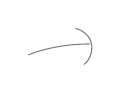
\begin{tikzpicture}\draw[gray] (0,0) .. controls (.24,.10) and (.54,.14) .. (.78,.14); \draw[gray] (.60,.34) .. controls (.89,.25) and (.83,-.03) .. (.71,-.12);\end{tikzpicture}}

Et la commutativité de (1) signifie la commutativité de (2) \uline{pour les objets}. Mais bien sûr on la veut aussi pour les flèches, i.e. on veut la commutativité du diagramme. $*$

% slanted
\margin{Donner l'exemple des morphismes de dérivateurs, définis par \unsure{des} foncteurs \tikz[baseline=(m.base)]\node[draw=gray,ellipse,inner sep=1pt] (m) {\unsure{sur|entre}}; des Cat. de modèles $(\unsure{\mathcal M|\mathscr M},\Sigma)\unsure{\longrightarrow|-}(\mathcal M',\Sigma')$}

Sans doute on veut un peu plus sur les morphismes de dérivateurs -- on veut une commutation aux $f_{*}$ et \inserted{(?)} aux $f_{!}$ (cette fois seulement iso. can. près) \ldots

% slanted
\margin{Commutation \unsure{à|:} \unsure{$f_{*}$ (resp. à $f_{!}$)} : morphisme \uline{exact à g.} (resp. à droite), les morphismes \uline{\unsure{exacts|existent}} sont \unsure{ceux} à la fois exacts \unsure{à g.} et à \unsure{dr.}}

% archive sheet number: 16
